\documentclass[conference]{IEEEtran}
\IEEEoverridecommandlockouts

\usepackage[utf8]{inputenc}
\usepackage[T1]{fontenc}
\usepackage[brazil]{babel}
\usepackage{cite}
\usepackage{amsmath,amssymb,amsfonts}
\usepackage{graphicx}
\graphicspath{{../results/experiments/plots/}{results/experiments/plots/}}
\usepackage{textcomp}
\usepackage{xcolor}
\usepackage{booktabs}
\usepackage{url}

\renewcommand{\abstractname}{Resumo}
\renewcommand{\IEEEkeywordsname}{Palavras-chave}

\begin{document}

\title{Simulação e Avaliação de Algoritmos de Escalonamento de Processos: uma Comparação entre FCFS, Round Robin, Prioridade e AHR}

\author{
\IEEEauthorblockN{Carlos Eduardo Bezerra Santos, David Josué Vital Santos, Henrique Coimbra Magalhães Filho e Levi Farias Leite}
\IEEEauthorblockA{\textit{Engenharia de Software -- Sistemas Operacionais}\\
\textit{Universidade Federal do Cariri (UFCA)}\\
Professor: WESKLEY VINICIUS FERNANDES MAURICIO\\
Brasil}
}

\maketitle

\begin{abstract}
O escalonamento de CPU envolve compromissos entre desempenho, justiça e custo de alternância entre processos. Este trabalho apresenta um simulador de escalonamento em C, com tempo discreto, chegadas reprodutíveis por seed, rajadas alternadas de CPU e E/S, bloqueio, preempção e custo explícito de troca de contexto. Foram implementados FCFS, Round Robin, Prioridade não preemptiva e um algoritmo próprio, denominado AHR (Aging com Histórico de Rajadas). O AHR combina prioridade base, tempo de espera e média das rajadas de CPU já observadas, sem consultar informação futura. A avaliação utiliza quatro cenários de carga, 100 seeds por cenário e 1.000 processos por execução, totalizando 1.600 execuções. As métricas são turnaround médio, trocas de contexto e índice de Jain aplicado ao slowdown, apresentadas com média e intervalo de confiança de 95\%. Os resultados mostram que Prioridade reduz o turnaround, porém produz forte desigualdade de slowdown; Round Robin aumenta a justiça, com custo elevado em turnaround e trocas no cenário CPU-bound; e o AHR recupera grande parte da justiça perdida pela Prioridade, mantendo custo de troca próximo aos algoritmos não preemptivos e comportamento de turnaround semelhante ao FCFS.
\end{abstract}

\begin{IEEEkeywords}
escalonamento de processos, simulação, Round Robin, prioridade, aging, índice de Jain, sistemas operacionais
\end{IEEEkeywords}

\section{Introdução}
O escalonador de CPU decide qual processo pronto utilizará o processador e, por consequência, influencia diretamente tempo de conclusão, responsividade e distribuição do atraso entre os processos. Algoritmos clássicos evidenciam que não existe uma única política superior em todos os objetivos: estratégias orientadas a trabalhos curtos podem reduzir turnaround, enquanto políticas preemptivas tendem a melhorar responsividade e justiça ao custo de mais alternâncias de contexto \cite{ostep}.

Este trabalho investiga esses compromissos por meio de um simulador reprodutível. Em vez de comparar os algoritmos em uma única carga, são utilizados cenários com perfis distintos de CPU, E/S e prioridades, sempre preservando a mesma carga para todos os escalonadores de uma combinação de cenário e seed. Além de FCFS, Round Robin (RR) e Prioridade não preemptiva, foi desenvolvido o AHR -- \textit{Aging com Histórico de Rajadas}. O algoritmo procura reduzir o risco de processos pouco prioritários permanecerem excessivamente prejudicados, sem recorrer ao conhecimento da próxima rajada de CPU.

A comparação é feita com três métricas complementares. O turnaround representa desempenho global; as trocas de contexto refletem o custo potencial da política; e o índice de Jain aplicado ao slowdown mede a igualdade relativa do atraso entre processos. Essa combinação é importante porque uma política pode produzir alta justiça simplesmente tornando todos igualmente lentos, ou reduzir o turnaround médio concentrando o prejuízo em um subconjunto de processos.

As principais contribuições são: (i) um motor único em C para quatro políticas de escalonamento; (ii) um gerador determinístico de cargas com quatro cenários; (iii) o AHR, que combina aging e histórico observado; e (iv) uma avaliação com 1.600 execuções e intervalos de confiança de 95\%.

\section{Modelo de Simulação}
\subsection{Tempo, estados e rajadas}
A simulação utiliza tempo discreto em ticks. Cada processo possui PID, instante de chegada, prioridade e uma sequência alternada de rajadas
\[
\mathrm{CPU}\rightarrow\mathrm{E/S}\rightarrow\mathrm{CPU}\rightarrow\cdots\rightarrow\mathrm{CPU}.
\]
Os estados são \texttt{NEW}, \texttt{READY}, \texttt{RUNNING}, \texttt{BLOCKED} e \texttt{FINISHED}. No início de cada tick, concluem-se operações de E/S, processos desbloqueados retornam a \texttt{READY} e novas chegadas são admitidas. Caso a CPU esteja livre, a política escolhe um processo; após eventual troca de contexto, executa-se um tick de CPU. Ao fim do tick são processados término de rajada, bloqueio, finalização ou preempção.

As operações de E/S são independentes e podem ocorrer em paralelo. Não existe dispositivo compartilhado nem fila de E/S no modelo principal: cada processo bloqueado aguarda apenas a duração de sua própria rajada. Essa simplificação isola o efeito do escalonamento de CPU, mas reduz a fidelidade em relação a sistemas nos quais processos disputam dispositivos de E/S.

\subsection{Troca de contexto e desempates}
A troca de contexto custa 2 ticks em todos os experimentos principais. Durante esse período a CPU não executa rajadas. A troca é contabilizada quando um processo deixa a CPU e outro processo diferente passa a executar; a transição de CPU ociosa para um processo não gera custo nem incrementa o contador.

A prioridade usa a convenção de que 0 é o valor mais prioritário. O FCFS preserva a ordem de entrada na fila de prontos; o RR utiliza a ordem circular da fila; a Prioridade seleciona o menor valor numérico e, em empate, preserva a ordem de prontidão. O AHR também mantém a ordem da fila em empates de seu score. Essas regras tornam a execução determinística para uma mesma carga.

\section{Algoritmos de Escalonamento}
\subsection{Algoritmos clássicos}
O \textbf{FCFS} é não preemptivo e escolhe o primeiro processo da fila de prontos. O \textbf{Round Robin} utiliza a mesma fila FIFO, mas preempta um processo quando ele consome o quantum configurado; neste estudo, $q=4$ ticks. Se a rajada termina ou bloqueia antes do limite, não é criada uma preempção artificial. A política de \textbf{Prioridade} também é não preemptiva e escolhe, sempre que a CPU fica livre, o processo \texttt{READY} com menor valor numérico de prioridade. A chegada de um processo mais prioritário não interrompe quem já está executando. Essas políticas representam compromissos clássicos entre turnaround, compartilhamento do processador e prioridades \cite{ostep}.

\subsection{AHR: Aging com Histórico de Rajadas}
O AHR foi projetado para mitigar a desigualdade causada pela prioridade estática sem abandonar completamente a prioridade original. A inspiração combina duas ideias conhecidas: aumentar gradualmente a preferência de processos que aguardam por muito tempo e utilizar comportamento passado para inferir características de execução \cite{ostep}. A diferença central é que o AHR não consulta a duração real da rajada atual ou de rajadas futuras.

Para cada processo pronto, define-se o histórico $h_i$ como a média inteira das rajadas de CPU já concluídas. Se nenhuma rajada foi concluída, usa-se uma estimativa inicial de 8 ticks. O tempo de espera atual é $w_i=\max(0,t-r_i)$, em que $t$ é o tempo atual e $r_i$ é o instante da última entrada em \texttt{READY}. O score é
\begin{equation}
S_i = 8p_i + h_i - \left\lfloor\frac{w_i}{4}\right\rfloor,
\label{eq:ahr}
\end{equation}
em que $p_i$ é a prioridade base. O processo com menor $S_i$ é selecionado. Assim, prioridades melhores reduzem a desvantagem inicial, histórico de rajadas curtas favorece processos que já demonstraram menor demanda de CPU e o termo de aging diminui continuamente o score de quem espera.

O AHR é não preemptivo: o score só é reavaliado quando a CPU volta a ficar disponível. Essa decisão evita gerar trocas adicionais em resposta a pequenas variações de score. Entre suas limitações estão a estimativa inicial fixa, a adaptação lenta quando o comportamento de um processo muda de fase e a sensibilidade aos pesos empíricos. Além disso, uma rajada longa já iniciada não pode ser interrompida pelo aging.

\section{Metodologia Experimental}
As cargas são geradas deterministicamente a partir de uma seed. O primeiro processo chega no tick 0 e os demais acumulam intervalos aleatórios de 0 a 3 ticks. As seeds utilizadas são os inteiros de 1 a 100. Para cada cenário e seed são executados os quatro algoritmos com 1.000 processos, resultando em $4\times100\times4=1.600$ execuções. Como o gerador é determinístico, a mesma combinação de seed e cenário produz a mesma carga para todas as políticas.

A Tabela~\ref{tab:cenarios} apresenta os parâmetros congelados dos quatro cenários. No cenário de prioridades desbalanceadas, 80\% das prioridades são sorteadas entre 0 e 1; nos demais, a distribuição de 0 a 9 é uniforme.

\begin{table*}[t]
\caption{Parâmetros dos cenários de carga. Todos os intervalos são inclusivos.}
\label{tab:cenarios}
\centering
\scriptsize
\begin{tabular}{lccccccl}
\toprule
\textbf{Cenário} & \textbf{Interchegada} & \textbf{Prioridade} & \textbf{Rajadas CPU} & \textbf{CPU (ticks)} & \textbf{E/S (ticks)} & \textbf{Viés} \\
\midrule
Equilibrado & 0--3 & 0--9 & 1--5 & 4--12 & 4--12 & uniforme \\
I/O-bound & 0--3 & 0--9 & 2--6 & 1--4 & 10--30 & uniforme \\
CPU-bound & 0--3 & 0--9 & 1--3 & 15--40 & 1--5 & uniforme \\
Prioridades desbalanceadas & 0--3 & 0--9 & 1--5 & 4--12 & 4--12 & 80\% em 0--1 \\
\bottomrule
\end{tabular}
\end{table*}

Para um processo $i$, o turnaround é
\begin{equation}
T_i=f_i-a_i,
\end{equation}
onde $f_i$ e $a_i$ são os instantes de término e chegada. O tempo ideal $I_i$ é a soma de todas as rajadas de CPU e E/S originais, isto é, o tempo do processo sem espera na fila de prontos. O slowdown é $x_i=T_i/I_i$. A justiça é medida pelo índice de Jain \cite{jain}:
\begin{equation}
J=\frac{\left(\sum_{i=1}^{n}x_i\right)^2}{n\sum_{i=1}^{n}x_i^2}.
\label{eq:jain}
\end{equation}
Valores próximos de 1 indicam slowdowns mais semelhantes. Para cada cenário, algoritmo e métrica foram calculados média, desvio padrão amostral $s$ e intervalo de confiança de 95\%,
\begin{equation}
IC_{95\%}=\bar{x}\pm1{,}96\frac{s}{\sqrt{n}}, \quad n=100.
\end{equation}

\section{Resultados}
A Tabela~\ref{tab:resultados} resume as médias das 100 seeds. As Figs.~\ref{fig:turnjain} e \ref{fig:switches} apresentam as mesmas médias com IC95\%. Os intervalos são estreitos em relação às diferenças mais pronunciadas entre políticas, indicando baixa variabilidade entre seeds para as tendências principais.

\begin{table*}[t]
\caption{Resultados médios dos experimentos principais ($n=100$ seeds por combinação). Jain é apresentado em porcentagem.}
\label{tab:resultados}
\centering
\scriptsize
\begin{tabular}{llrrr}
\toprule
\textbf{Cenário} & \textbf{Algoritmo} & \textbf{Turnaround (ticks)} & \textbf{Trocas} & \textbf{Jain (\%)} \\
\midrule
Equilibrado & FCFS       & 18.095,6 & 2.995,0 & 79,46 \\
            & RR         & 24.977,9 & 6.987,6 & 85,18 \\
            & Prioridade & 14.628,1 & 2.995,0 & 34,75 \\
            & AHR        & 18.076,9 & 2.995,0 & 79,39 \\
\midrule
I/O-bound   & FCFS       & 12.031,4 & 4.003,2 & 86,57 \\
            & RR         & 12.031,4 & 4.003,2 & 86,57 \\
            & Prioridade &  8.637,1 & 4.003,2 & 51,15 \\
            & AHR        & 11.987,7 & 4.003,2 & 86,12 \\
\midrule
CPU-bound   & FCFS       & 35.045,0 & 1.994,0 & 85,05 \\
            & RR         & 60.143,0 & 14.424,3 & 96,48 \\
            & Prioridade & 29.353,7 & 1.994,0 & 55,99 \\
            & AHR        & 35.049,6 & 1.994,0 & 85,05 \\
\midrule
Prioridades desbal. & FCFS       & 18.120,1 & 2.996,2 & 79,61 \\
                    & RR         & 25.023,7 & 6.995,0 & 85,27 \\
                    & Prioridade & 15.600,1 & 2.996,2 & 36,89 \\
                    & AHR        & 18.109,1 & 2.996,2 & 79,51 \\
\bottomrule
\end{tabular}
\end{table*}

\begin{figure*}[t]
\centering
\begin{minipage}{0.49\textwidth}
\centering
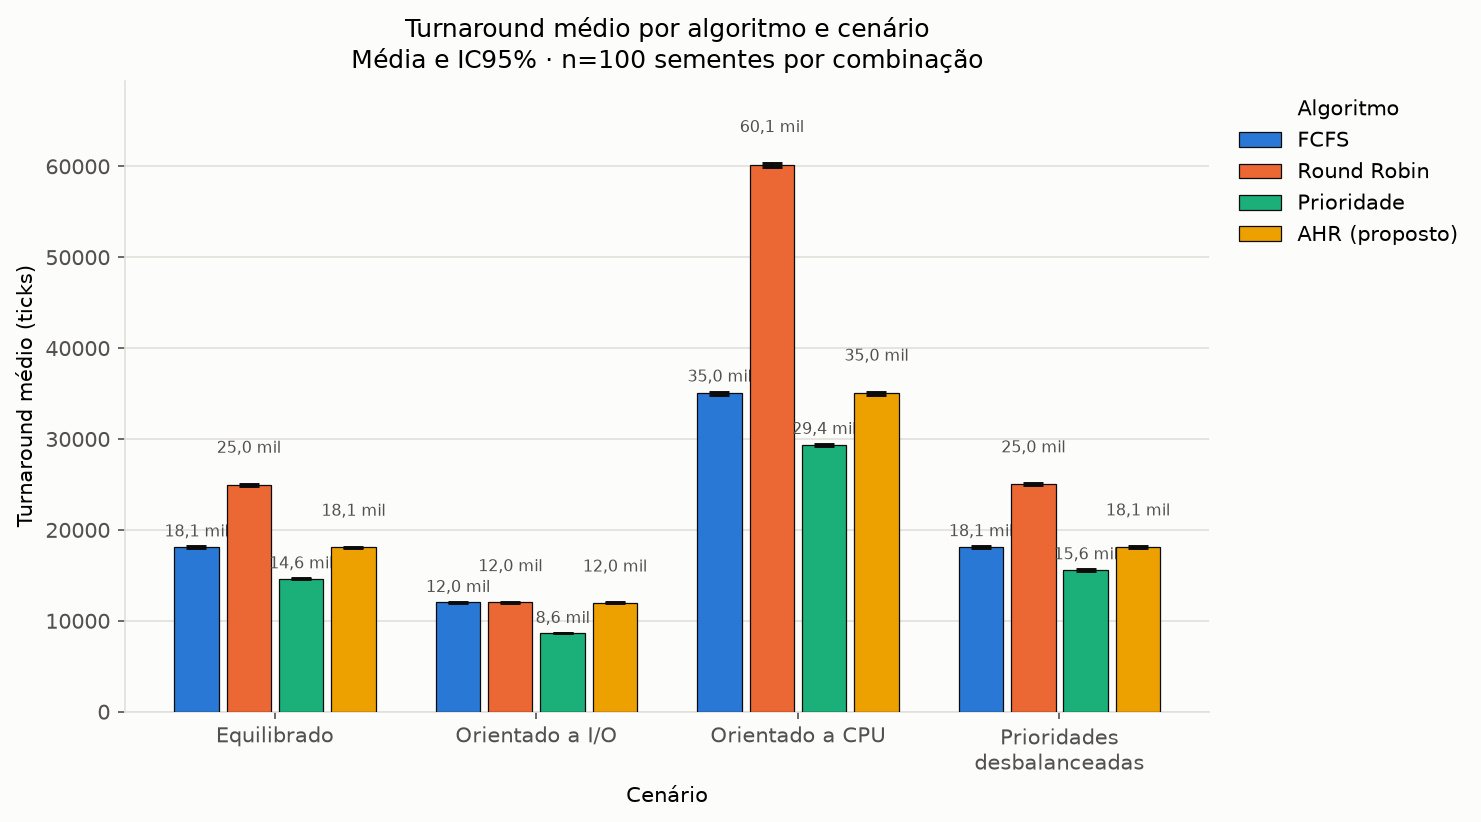
\includegraphics[width=\linewidth]{turnaround_medio.png}\\[-1mm]
{\footnotesize (a) Turnaround médio.}
\end{minipage}\hfill
\begin{minipage}{0.49\textwidth}
\centering
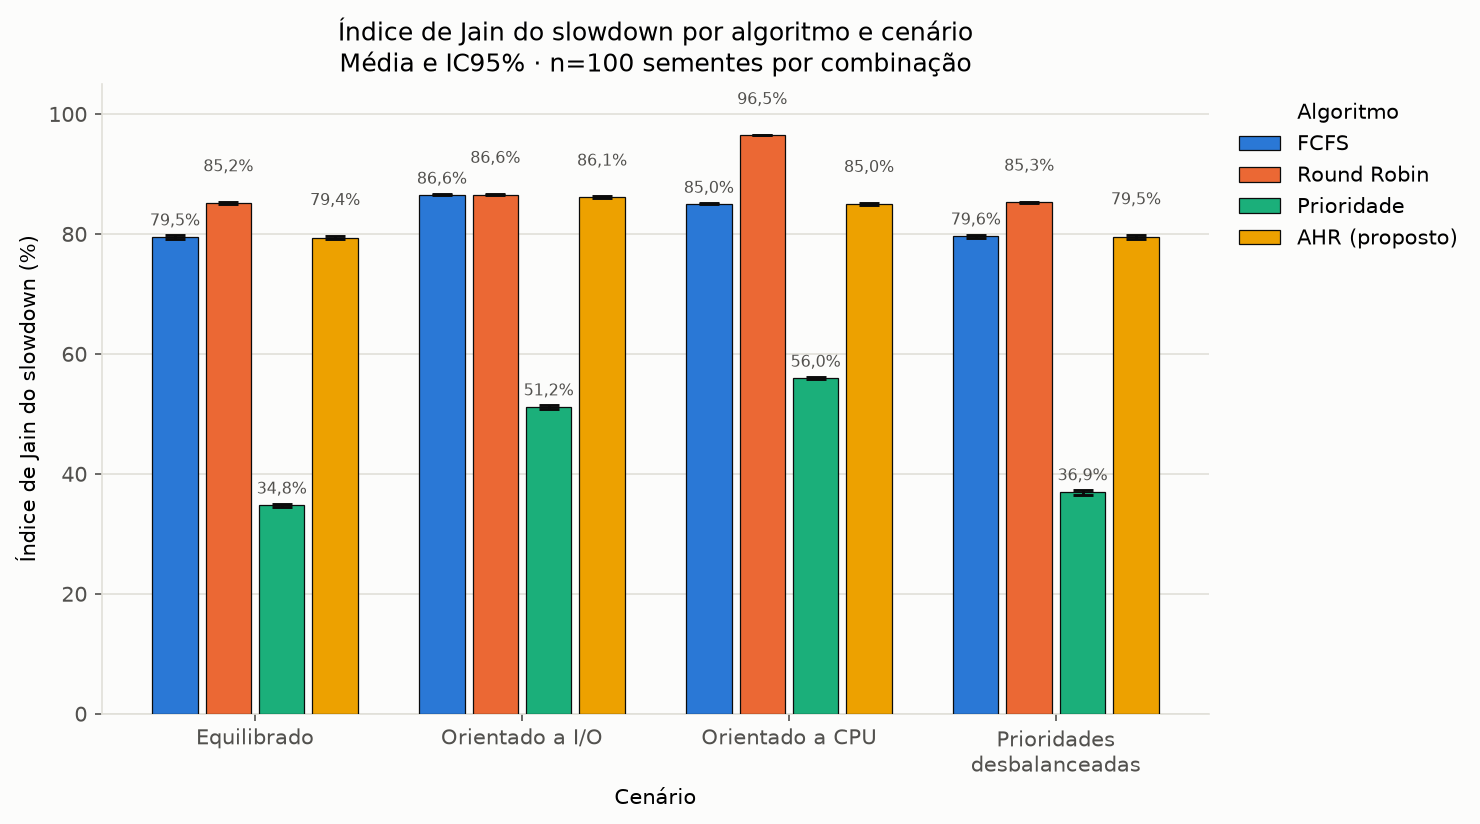
\includegraphics[width=\linewidth]{jain_slowdown.png}\\[-1mm]
{\footnotesize (b) Índice de Jain aplicado ao slowdown.}
\end{minipage}
\caption{Desempenho e justiça por cenário. As barras representam a média de 100 seeds e as hastes indicam IC95\%.}
\label{fig:turnjain}
\end{figure*}

\begin{figure}[t]
\centering
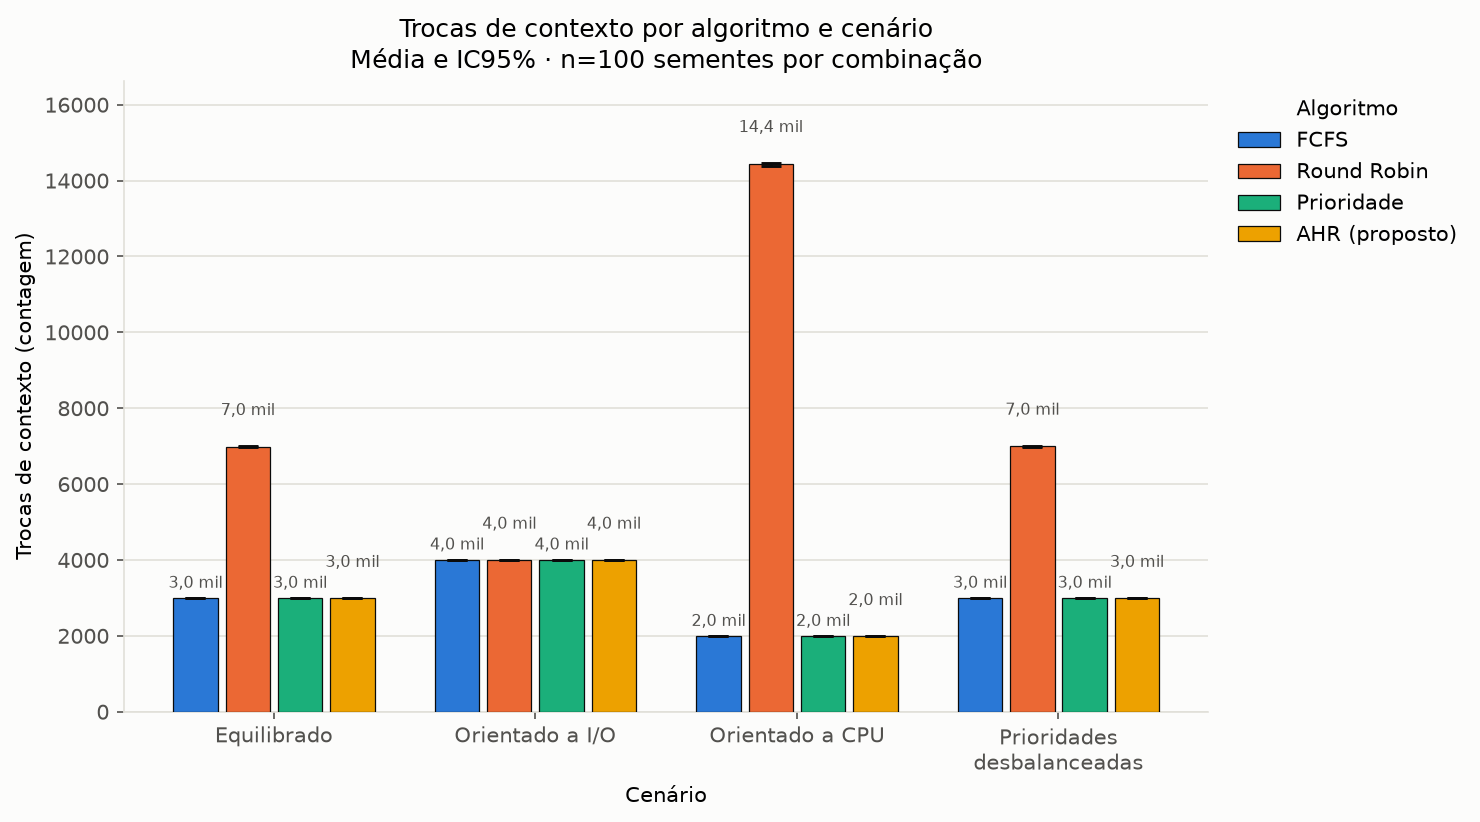
\includegraphics[width=\columnwidth]{trocas_contexto.png}
\caption{Número médio de trocas de contexto, com IC95\% e 100 seeds por combinação.}
\label{fig:switches}
\end{figure}

A política de Prioridade obteve o menor turnaround em todos os cenários. No equilibrado, sua média foi 14.628,1 ticks, contra 18.076,9 do AHR; no CPU-bound, 29.353,7 contra 35.049,6. Entretanto, esse ganho veio acompanhado de forte queda de justiça: Jain de 34,75\% no equilibrado e 36,89\% nas prioridades desbalanceadas. O comportamento é coerente com uma política que favorece repetidamente os processos de maior prioridade e concentra a espera nos demais.

O AHR alterou esse compromisso. No cenário de prioridades desbalanceadas, atingiu Jain de 79,51\%, aumento de 42,62 pontos percentuais em relação à Prioridade, enquanto o turnaround subiu 16,1\%. No equilibrado, a justiça também aumentou de 34,75\% para 79,39\%, com aumento de 23,6\% no turnaround em relação à Prioridade. Em todos os cenários, o turnaround e o Jain do AHR ficaram muito próximos aos do FCFS; portanto, a hipótese de recuperar justiça em relação à Prioridade foi confirmada, mas não houve ganho adicional relevante sobre o FCFS na configuração adotada.

O RR apresentou a maior justiça nos cenários equilibrado, CPU-bound e de prioridades desbalanceadas. O maior contraste ocorreu no CPU-bound: Jain de 96,48\%, mas turnaround de 60.143,0 ticks, 71,6\% acima do AHR. Além disso, o RR realizou em média 14.424 trocas contra 1.994 do AHR, aproximadamente 7,2 vezes mais. Isso decorre das rajadas de CPU entre 15 e 40 ticks, muito maiores que o quantum 4, o que provoca preempções frequentes.

No cenário I/O-bound ocorre um caso de controle útil: as rajadas de CPU variam de 1 a 4 ticks, nunca excedendo o quantum principal do RR. Consequentemente, RR e FCFS apresentaram exatamente as mesmas médias nas três métricas. O resultado confirma que, sem expiração de quantum, a preempção do RR deixa de atuar e a política se comporta como uma fila FIFO. O AHR reduziu o turnaround em apenas 0,36\% frente ao FCFS, com Jain 0,45 ponto percentual menor.

\section{Discussão}
Os resultados evidenciam que a escolha do escalonador não pode ser reduzida a uma única métrica. A Prioridade foi a melhor política em turnaround, inclusive quando as prioridades eram desbalanceadas, porém sua justiça foi a pior em todos os cenários. Essa política é adequada quando a prioridade representa uma preferência que deve realmente dominar a execução, mas é problemática quando se deseja evitar que processos menos prioritários sofram atrasos proporcionalmente muito maiores.

O AHR cumpre parcialmente o objetivo proposto. O termo de aging compensa progressivamente a prioridade ruim e elevou de forma expressiva a justiça em relação à Prioridade. Ao mesmo tempo, por ser não preemptivo, não introduziu a explosão de trocas observada no RR. No cenário de prioridades desbalanceadas, por exemplo, o AHR manteve cerca de 79,5\% de Jain com aproximadamente 2.996 trocas, enquanto o RR chegou a 85,3\% com cerca de 6.995 trocas. O AHR, portanto, oferece um ponto intermediário: perde parte da justiça do RR, mas evita sua sobrecarga e reduz substancialmente o turnaround em relação a ele.

Por outro lado, a semelhança entre AHR e FCFS revela uma limitação importante. Os pesos $8$, $1$ e o intervalo de aging de 4 ticks foram congelados antes da bateria final, evitando ajuste oportunista por cenário, mas a combinação escolhida fez com que a política se aproximasse de uma ordenação guiada pelo tempo de espera em grande parte das cargas. O histórico médio de CPU não produziu uma vantagem consistente de turnaround sobre o FCFS. Uma análise futura de sensibilidade poderia variar os pesos em uma grade fixa, separada dos resultados principais, para verificar se existe uma região que preserve a justiça observada e aumente a influência do histórico.

Também é necessário considerar as limitações do modelo. O simulador possui uma única CPU, E/S paralela sem contenção por dispositivo e distribuições sintéticas. Assim, os números absolutos não devem ser interpretados como previsão de desempenho de um sistema operacional real. O objetivo é comparar políticas sob condições controladas e reproduzíveis. Ainda assim, os padrões observados -- preempção elevando trocas, prioridade reduzindo turnaround com perda de justiça e aging recuperando processos desfavorecidos -- são compatíveis com os compromissos esperados em escalonamento de CPU \cite{ostep}.

\section{Conclusão}
Foi desenvolvido um simulador reprodutível de escalonamento de processos e comparadas quatro políticas em 1.600 execuções. A Prioridade não preemptiva apresentou o menor turnaround, mas baixa justiça de slowdown. O Round Robin apresentou os maiores índices de Jain, porém tornou-se caro em workloads CPU-bound devido ao grande número de preempções e trocas de contexto. O AHR atingiu o objetivo principal de reduzir a desigualdade da Prioridade sem aumentar as trocas em relação às políticas não preemptivas. Em prioridades desbalanceadas, seu Jain foi 79,51\%, contra 36,89\% da Prioridade, ao custo de turnaround 16,1\% maior. Entretanto, seu comportamento ficou próximo ao FCFS, indicando que os parâmetros e o uso do histórico ainda oferecem espaço para investigação. Os resultados reforçam que desempenho, justiça e custo de escalonamento devem ser interpretados conjuntamente e sempre em função do perfil da carga.

\begin{thebibliography}{00}
\bibitem{ostep}
R. H. Arpaci-Dusseau and A. C. Arpaci-Dusseau, \textit{Operating Systems: Three Easy Pieces}, Version 1.10. Arpaci-Dusseau Books, Nov. 2023.

\bibitem{jain}
R. Jain, D. Chiu, and W. Hawe, ``A Quantitative Measure of Fairness and Discrimination for Resource Allocation in Shared Computer Systems,'' Digital Equipment Corporation, DEC Research Report TR-301, Sep. 1984.
\end{thebibliography}

\end{document}
